\documentclass[10pt,a4paper]{book}
\usepackage[utf8]{inputenc}
\usepackage[english]{babel}
\usepackage{amsmath}
\usepackage{amsfonts}
\usepackage{stmaryrd}
\usepackage{amssymb}
\usepackage{amsthm}
\usepackage{graphicx}
\usepackage{tikz}
\usepackage{physics}
\usepackage[left=2cm,right=2cm,top=2cm,bottom=2cm]{geometry}
\author{Marco Biroli}
\title{Probability}


\newtheorem{theorem}{Theorem}[section]
\newtheorem{corollary}{Corollary}[theorem]
\newtheorem{lemma}[theorem]{Lemma}
\newtheorem{proposition}{Proposition}[section]

\newtheorem*{remark}{Remark}
\newtheorem*{notation}{Notation}

\theoremstyle{definition}
\newtheorem{definition}{Definition}[section]


\begin{document}
\maketitle
\tableofcontents
\chapter{Founding Blocks}
\section{Definitions}

\begin{definition}[Universe]
We consider a random experiment, then the set of all possible outcomes of the experiment is denoted by $\Omega$ and is called the universe.
\end{definition}

\begin{definition}[Event]
An event is usually denoted by $E$. An event is a set of results for which we can compute the probability.
\end{definition}

\begin{definition}[Collection]
The collection of all events is denoted by $\mathcal{F}$. Hence $\mathcal{F} \subseteq \mathcal{P}(\Omega)$.
\end{definition}

\begin{definition}[Disjoint Events]
Two events $A, B \in \mathcal{F}$ are disjoint or incompatible if they cannot occur simultaneously. In other words if $A \cap B = \emptyset$.
\end{definition}

\begin{remark}
We require that the collection $\mathcal{F}$ of the events is an algebra of sets.
\end{remark}

\begin{definition}[Algebra of Sets]
An element $\mathcal{F}$ is called an algebra of sets if $\mathcal{F} \neq \emptyset$ and:
\begin{enumerate}
\item $A \in \mathcal{F} \Rightarrow A^c \in \mathcal{F}$
\item $A, B \in \mathcal{F} \Rightarrow A \cup B \in \mathcal{F}$
\end{enumerate}
\end{definition}

\begin{remark}
For the scope of this course we further require that $\mathcal{F}$ is stable under countable unions. In other words the second condition above is replaced by:
\[
(A_n)_{n \in \mathbb{N}} \in \mathcal{F}^\mathbb{N} \Rightarrow \bigcup_{n \in \mathbb{N}} A_n \in \mathcal{F}
\]
\end{remark}

\begin{definition}[$\sigma$-algebra]
A $\sigma$-algebra is an algebra of sets where the second condition is replaced by the stronger condition requiring stability under countable union.
\end{definition}

\begin{definition}[Probability]
The probability $P(E)$ of $E$ is the theoretical value for the proportion of experiments in which $E$ occurs. Thus the probability is a function from $\mathcal{F}$ to $[0,1]$. Such that:
\begin{enumerate}
\item $P(\Omega) = 1$.
\item $A, B \in \mathcal{F}, A \cap B = \emptyset \Rightarrow P(A \cup B) = P(A) + P(B)$.
\end{enumerate}
In other words, $P$ is an additive set function from $\mathcal{F}$ to $[0,1]$.
\end{definition}

\begin{remark}
This definition however is not very well suited to infinite event sets. Then modern probability theory adds a condition to the above.
\end{remark}

\begin{definition}[Modern Probability]
A modern probability $P(E)$ of $E$ is a probability with the stronger condition:
\[
\forall (A_n)_{n \in \mathbb{N}} \in \mathcal{F}^\mathbb{N}, \left(\forall n, m \in \mathbb{N}, n \neq m \Rightarrow A_n \cap A_m = \emptyset\right) \Rightarrow P\left(\bigcup_{n \in \mathbb{N}} A_n \right) = \sum_{n \in \mathbb{N}} P(A_n)
\]
\end{definition}

\begin{definition}[Probability Space]
A probability space is a triple $(\Omega, \mathcal{F}, P)$. Where $\Omega$ is the universe of all possible results, $\mathcal{F}$ is a $\sigma$-field on $\Omega$, and $P$ is a modern probability function on $\mathcal{F}$.
\end{definition}

\begin{remark}
The mathematical framework which defines probability theory actually comes from another mathematical framework called measure theory. This is why the elements of the $\sigma$-field are sometimes called the measurable sets and the probability function is sometimes called a probability measure.
\end{remark}

\begin{definition}[Finite Space]
We consider the case where $\Omega$ is a finite set, we write $\Omega = \{x_1, \ldots, x_n\}$. The natural $\sigma$-field on $\Omega$ is $\mathcal{P}(\Omega)$. It is the only $\sigma$-field which contains the singletons. Then let $P$ be a probability on $\Omega$ and let us set $\forall i \in \llbracket 1, n\rrbracket, p_i = P(\{x_i\})$. Then the numbers $p_i$ satisfy:
\[
\left( \forall i \in \llbracket 1, n\rrbracket, 0 \leq p_i \leq 1\right) \land \sum_{i = 1}^n p_i = 1
\]
Then for any $A \subset \Omega$ we have by additivity that:
\[
P(A) = \sum_{x \in A} P(\{x\}) = \sum_{i : x_i \in A} p_i
\]
Hence $P$ is completely determined by the numbers $p_i$.
\end{definition}

\begin{remark}
Notice that conversely if we are given the numbers $p_i$ summing to 1 we can define a probability $P$ on $\Omega$ by stating $P(\{x_i\}) = p_i$ and $P$ will indeed be a probability measure.
\end{remark}

\begin{definition}[Countable Spaces]
We suppose that $\Omega$ is countable and we set $\Omega = \{ x_n , n \in \mathbb{N}\}$. The natural $\sigma$-field on $\Omega$ is again the power set of $\Omega$. Then the definitions are an immediate generalization of the ones for a finite space.
\end{definition}

\begin{definition}[Continuous Spaces]
If we take the simplest example of $\Omega = \mathbb{R}$ then the intuitive $\sigma$-field being the power set turns out to be too complicated to be useful. Hence we take for $\mathcal{F}$ the Borel tribe of $\mathbb{R}$, $\mathcal{B}(\mathbb{R})$. The Borel $\sigma$-field corresponds to taking a countable union of all possible closed intervals of $\mathbb{R}$.
\end{definition}

\begin{definition}[Random Variable]
Let $(\Omega, \mathcal{F}, P)$ be a probability space. A random variable $X$ on $(\Omega, \mathcal{F}, P)$ is map from $\Omega$ to $\mathbb{R}$. Which satisfies:
\[
\forall B \in \mathcal{B}(\mathbb{R}), X^{-1}(B) = \{ \omega \in \Omega : X(\omega) \in B \} \in \mathcal{F}
\]
\end{definition}

\begin{remark}
This definition is equivalent to: for all interval $I$ of $\mathbb{R}$ we have that $X^{-1}(I) \in \mathcal{F}$.
\end{remark}

\begin{notation}
The event $X^{-1}(I)$ is denoted by $\{X \in I\}$ or even simply $X \in I$. Secondly random variables are denoted by capital letters typically $X, Y, U, V$ and their possible values are denoted by the corresponding lowercase letters.
\end{notation}

\begin{definition}[Law of a random variable]
Let $(\Omega, \mathcal{F}, P)$ be a probability space and let $X$ be a random variable defined on $\Omega \to \mathbb{R}$. The law of $X$ is the probability measure on $\mathbb{R}$ defined by:
\[
\forall B \in \mathcal{B}(\mathbb{R}), P_X(B) = P(X \in B)
\]
\end{definition}

\begin{proof}
Let us check that $P_X$ is indeed a probability measure. We have that:
\[
P_X(\mathbb{R}) = P(X \in \mathbb{R}) = 1.
\]
Furthermore let $(B_n)_{n \in \mathbb{N}} \in \mathcal{B}(\mathbb{R})^\mathbb{N}$ be a disjoint sequence of Borel sets. Then:
\[
P_X\left(\bigcup_{n \in \mathbb{N}} B_n\right) = P\left(X \in \bigcup_{n\in\mathbb{N}} B_n\right) = P\left( \bigcup_{n\in\mathbb{N}} \{ X \in B_n \} \right) = \sum_{n \in \mathbb{N}} P(X \in B_n) = \sum_{n \in \mathbb{N}} P_X(B_n)
\]
\end{proof}

\begin{notation}
The law $P_X$ of $X$ is sometimes called the \textit{distribution} of $X$. We furthermore say that two variables $X, Y$ have the same law if $P_X = P_Y$. The object of primary interest for a random variable is its law.
\end{notation}

\begin{definition}[Law]
Let $f$ be a non-negative function $\mathbb{R} \to \mathbb{R}^+$ which is integrable and $\int_\mathbb{R} f(x) \dd x = 1$. We define next:
\[
\forall A \in \mathcal{B}(\mathbb{R}) \quad P(A) = \int_A f(x) \dd x
\]
This formula defines a probability measure on $\mathbb{R}$, called the probability measure with density function $f$.
\end{definition}

\begin{definition}[Expectation]
We say that the random variable $X$ has an expectation or that it is integrable if:
\[
\int_\mathbb{R} |x| \dd P_X(x) < +\infty
\]
Then the expectation is defined as:
\[
E(X) = \int_\mathbb{R} x \dd P_X(x) = \int_\Omega X \dd P = \int_{\omega \in \Omega} X(\omega)\dd P(\omega) = \int_\mathbb{R} \text{Id}_\mathbb{R} \dd P_X
\]
From this formula we see that the expectation is completely dependent on the law of the random variable.
\end{definition}

\chapter{Coin tossing games.}

\section{The model}
We take a fair coin and consider the experiment which consists in throwing $n$ times the coin.If -1 denotes tail and +1 denotes head then the result of the experiment is $r \in \{-1, 1\}^n = \Omega$. Since $\Omega$ is finite we immediately have $\mathcal{F} = \mathcal{P}(\Omega)$. Since we assumed the coin to be fair we have by symmetry that all the results are equiprobable. Hence:
\[
\forall \omega \in \Omega, \quad P(\omega) = \frac{1}{|\Omega|} = \frac{1}{2^n}
\]
Now let $X_k$ be the random variable corresponding to the result of the $k$-th throw. Formally $X_k$ is the map:
\begin{align*}
X_k : \Omega &\longrightarrow  X_k(\Omega)\\
(\omega_1, \cdots, \omega_n) &\longmapsto \omega_k 
\end{align*}

\section{Graphical Representation.}
To the sequence $X_1, \cdots, X_n$ we associate the partial sums $S_0 = 0, S_1 = X_1, \cdots, S_n = X_1 + \cdots + X_n$. The sequence $S_0, \cdots, S_n$ contains exactly the same information as $X_1, \cdots, X_n$. We can therefore represent the result of the experiment by a polygonal line, which is the line which joins successively the points: $(0, S_0), \cdots, (n, S_n)$. Such a polygonal line, associated to a sequence of signs, will be called a path.

\section{Interpretation of the model.}
\subsection{Coin tossing game} Potter and Voldemort play the following game. Potter throws a coin and Voldemort tries to guess the result. If Voldemort is wrong he pays 1 euro to Potter however if he is right Potter gives 1 euro to Voldemort. Then $S_n$ represents the algebraic gain of Potter after $n$ turns. 
\subsection{Random Walk} We consider a drunkard which performs a random walk on $\mathbb{Z}$ with the following mechanism. At $t=0$ we center the origin on his position, then at every step he tosses a fair coin and he goes left or right according to whether he obtains tails or heads. Then $S_n$ corresponds to the final position after $n$ steps.
\begin{figure}
\centering
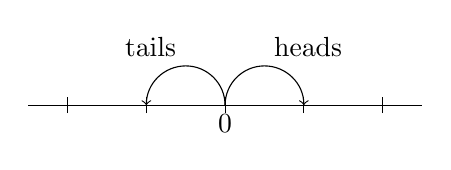
\begin{tikzpicture}
\draw (-2.5, 0) -- (2.5, 0);
\draw (0, 0) node[below] {0};
\draw (0, -0.1) -- (0, 0.1);
\draw (1, -0.1) -- (1, 0.1);
\draw (2, -0.1) -- (2, 0.1);
\draw (-1, -0.1) -- (-1, 0.1);
\draw (-2, -0.1) -- (-2, 0.1);
\draw[->] (0,0) arc(0:180:0.5);
\draw[<-] (1,0) arc(0:180:0.5);
\draw (0.5, 0.5) node[above right] {heads};
\draw (-0.5, 0.5) node[above left] {tails};
\end{tikzpicture}
\end{figure}

\section{Distribution or law of $S_n$}
\begin{proposition}
The law of $S_n$ is the probability distribution on $\{-n, \cdots, n\}$ given by:
\[
\forall k \in \{-n, \cdots, n\} \quad P(S_n = k) = \binom{n}{\frac{n + k}{2}} \frac{1}{2^n}
\]
\end{proposition}
\begin{proof}
A simple proof can be done geometrically. We know that all results are equiprobable hence it suffices to count the number of possible choice that leads to $S_n = k$. Let us consider such a path and let us denote by $\alpha$ the number of ascending steps and $\beta$ the number of descending steps, then we have that:
\[
\begin{cases}
\alpha - \beta = k\\
\alpha + \beta = n
\end{cases}
\Rightarrow \alpha = \frac{n + k}{2}
\] 
Then the number of possible paths is simply given by the number of possible choices for the ascending steps which are immediately given by: $\binom{n}{\alpha}$.
\end{proof}

\section{Equalization or return to 0} We say that there is an equalization or return to 0 at time $n$ if $S_n = 0$. Since $n$ and $S_n$ have the same parity this occurs only at even times. Then from what we got previously we immediately get that:
\[
P(S_{2n} = 0) = \frac{1}{2^{2n}} \binom{2n}{n} = \frac{1}{2^{2n}} \frac{(2n)!}{(n!)^2}
\]
Then Stirling's formula tells us that: $n! = \left(\frac{n}{\ell}\right)^n \sqrt{2\pi n} \left( 1 + \frac{1}{12 n} + \frac{1}{288 n^2} + o(\frac{1}{n^2})\right)$ and applying it above we obtain:
\[
P(S_{2n} = 0) \stackrel{n \to +\infty}{\sim} = \frac{1}{\sqrt{\pi n}}
\]
This gives an excellent approximation even for small values of $n$.

\section{The lamplighter walk.}
Imagine you have an infinite street with lanterns every meter and one lamplighter whose job is to light all the lanterns. He also starts at the origin and lights the lantern at the origin. Then he throws a coin and goes left or right according to if it is tails or heads and lights the successive lantern. The position at time $n$ is given by $S_n$ and the process $(S_n)_{n \in \mathbb{N}}$ is the symmetric random walk on $\mathbb{Z}$. Now we are interested in the following question: What is the probability that the lamplighter comes back to the original lantern? Mathematically this is described by:
\begin{align*}
P(\exists n \in \mathbb{N}^*, S_{2n} = 0) &= P\left(\bigcup_{n \geq 1} \{ S_{2n} = 0 \} \right) \\
&= P\left(\{S_2 = 0\} \cup (\{S_4 = 0\}\setminus\{S_2 = 0\}) \cup \cdots \cup (S_{2n = 0} \setminus (\{S_2 = 0\} \cup \cdots \cup \{S_{2n - 2} = 0\} )\right)\\
&= P\left(\bigcup_{n \geq 1} \left( \left\{S_{2n} = 0\right\} \setminus \left( \left\{S_2 = 0\right\} \cup \cdots \cup \left\{ S_{2n - 2} \right\} \right) \right)\right)
\end{align*}
Now since the events are disjoint we can use the $\sigma$-additivity property. Hence we get:
\[
P(\exists n \in \mathbb{N}^*, S_{2n} = 0) = \sum_{n \geq 1} P(S_2 \neq 0, \cdots, S_{2n - 2} \neq 0, S_{2n} = 0)
\]
Now necessarily all the $S_{2i}$ for $i \in \llbracket 1, n-1\rrbracket$ must have the same sign. By symmetry the probability that they are all positive is equal to the probability that they are all negative. Hence:
\begin{align*}
P(\exists n \in \mathbb{N}^*, S_{2n} = 0) &= 2 P(S_1 > 0, \cdots, S_{2n-1} > 0, S_{2n} = 0) \\
&= \frac{2}{2^{2n}} |\{ \text{paths from } (1, 1) \text{ to } (2n -1, 1) \text{ which do not touch the axis} \}|
\end{align*}
Now we decide to count the number of paths that do touch the axis instead of the one that do not touch the axis. Since we know the total number of paths this is an equivalent problem. 

\section{Reflection principle.} Let $A = (a, \alpha)$ and $B = (b, \beta)$ be two points with $0 < a < b$ and $\alpha, \beta > 0$. My problem now is to count the number of paths that go from $A$ to $B$ which touch or cross the axis. Notice that this problem is perfectly equivalent to counting the number of paths that go from $A' = (a, -\alpha)$ to $B$. To formalize this we need to make sure that this is a one-to-one map. Consider a path $s = (s_a, s_{a+1}, \cdots, s_b)$ be a path from $A$ to $B$ which touches the axis and $t$ be the first time it touches in other words $t = \min\{ i \geq a : s_i = 0\}$. Let $T = (t, 0)$ and to the path $s$ we associate the path $\phi(s)$ obtained from $s$ by taking the reflexion of the portion $AT$ with respect to the $x$-axis. Now we claim that $\phi$ is a one-to-one correspondence from the paths from $A$ to $B$ which touch the axis unto the paths from $A'$ to $B$. In fact $\phi$ is an involution ($\phi^2 = \text{Id}$) and hence it is injective and obviously surjective therefore bijective. 

\section{The ballot theorem.} Let $x, n > 0$. The number of paths from $(0,0)$ to $(n, x)$ which do not touch the axis after time $0$ is equal to the number of paths from $(1, 1)$ to $(n,x)$ minus the number of paths from $(1, -1)$ to $(n, x)$. This immediately yields:
\[
\frac{x}{n}\binom{n}{\frac{n+x}{2}}
\]  
An example of application is the following. In an election the candidate $P$ scores $p$ votes and $Q$ scores $q$ votes with $p > q$. The probability that the winning candidate is always ahead during the reading of the votes is given by:
\[
\frac{p - q}{p + q}
\]

\section{End of the computation.}
Now going back to our lamplighter computation applying the reflexion principle we have that:
\[
P(\exists n \in \mathbb{N}^*, S_{2n} = 0) = \frac{2}{2^{2n}} \frac{1}{2n - 1} \binom{2n - 1}{n} = \frac{1}{2n - 1} P(S_{2n} = 0)
\]
Hence the probability that the lamplighter returns to 0 is given by:
\[
P(\text{return to 0}) = \sum_{n \geq 1} \frac{1}{2n -1} P(S_{2n} = 0) = \sum_{n \geq 1} P(S_{2n - 2} = 0 ) - P(S_{2n} = 0) = 1
\]

\section{Fundamental Lemma}
From the previous computation we have gotten that:
\[
P(S_2 \neq 0, \cdots, S_{2n - 2}\neq 0, S_{2n} = 0) = P(S_{2n - 2} = 0) - P(S_{2n} = 0)
\]
Yet we also have that:
\[
P(S_2 \neq 0, \cdots, S_{2n - 2}\neq 0, S_{2n} = 0) = P(S_2 \neq 0, \cdots, S_{2n - 2}\neq 0) - P(S_2 \neq 0, \cdots, S_{2n - 2}\neq 0, S_{2n} \neq 0)
\]
Hence for any $n$ larger than 1 we have that:
\[
P(S_{2n - 2} = 0) - P(S_{2n} = 0) = P(S_2 \neq 0, \cdots, S_{2n - 2}\neq 0) - P(S_2 \neq 0, \cdots, S_{2n - 2}\neq 0, S_{2n} \neq 0)
\]
Moreover we have that:
\[
P(S_2 \neq 0 ) = \frac{1}{2} = P(S_2 = 0)
\]
Which gives the fundamental lemma:
\[
P(S_2 \neq 0, \cdots, S_{2n} \neq 0) = P(S_{2n} = 0)
\]

\section{Last tie}
Consider a coin tossing game of length $2n$ and the time $T$ of the last tie before $2n$: $T = \max\{k \leq 2n : S_k = 0\}$. Now we want to find the distribution of $T$. 
\begin{proposition}
The law of $T$ is called the arcsinus law and is given by:
\[
P(T = k) = P(S_{2k} = 0)P(S_{2n - 2k} = 0)
\]
\end{proposition}

\chapter{Independence} 

\section{Conditional Probability.}

Let $(\Omega, \mathcal{F}, P)$ be a probability space and $A, B \subset \mathcal{F}$ with $P(B) > 0$. Then we have that the conditional probability of A given B is as follows:
\[
P(A | B) = \frac{P(A \cap B)}{P(B)}
\]
This formula however does not hold in the general case where $P(B) = 0$ where the treatment is much more delicate. Now notice that $B$ being fixed the application $A \in \mathcal{F} \mapsto P(A|B)$ is a probability measure on $\mathcal{F}$. 

\section{Sub $\sigma$-field and generated $\sigma$-fields}
A sub $\sigma$-field  $\mathcal{G}$ of $\mathcal{F}$ is a $\sigma$-field $\mathcal{G}$ such that $\mathcal{G} \subset \mathcal{F}$. Now let $\mathcal{A}$ be a collection of parts of $\Omega$. The $\sigma$-field generated by $\mathcal{A}$ denoted by $\sigma(\mathcal{A})$ is the smallest $\sigma$-field on $\Omega$ which contains all the elements of $\mathcal{A}$. Formally it is defined as being the intersection of all the $\sigma$-fields which contain $\mathcal{A}$. Now let $E$ be a set equipped with a $\sigma$-field $\mathcal{E}$. Now we start by generalizing the concept of random variable. A random variable $X$ taking values in $E$ is a map $X : \Omega \to E$ such that:
\[
\forall A \in \mathcal{E}, \quad X^{-1}(A) = \left\{ \omega \in \Omega : X(\omega) \in A \right\} \in \mathcal{F}
\] 
Then formally the $\sigma$-field generated by the random variable $X$ is given by:
\[
\sigma(X) = \{ X^{-1}(A) : A \in \mathcal{E}\}
\]
We leave it as an exercise to the reader to check that this does indeed define a $\sigma$-field.

\section{Fundamental definition of independence}

\begin{definition}[Two independent events]
Let $(\Sigma, \mathcal{F}, P)$ be a probability space. Then 2 events $A, B \in \mathcal{F}$ are said to be independent if and only if $P(A \cap B) = P(A) P(B)$. 
\end{definition}

\begin{remark}
Notice right away that if $A, B$ are independent then $A, B^c$ are independent and so is $A^c, B^c$. Furthermore if $P(B) > 0$ then using the definition of conditional probability we can write it as $P(A | B) = P(A)$. This is a representation of the intuitive notion: "if $A$ does not depend on $B$ then the advent of $B$ should change nothing to result of $A$".  
\end{remark}

\begin{definition} [Multiple independent events] \label{indp:events} Consider $n$ events $A_1, \cdots, A_n$. They are said to be independent if and only for all finite subset $I$ of $\{1, \cdots, n\}$ we have:
\[
P\left( \bigcup_{i \in I} A_i \right) = \prod_{i \in I} P(A_i)
\]
\end{definition}

\begin{remark}
Notice that this statement is much stronger than the one requiring for the events to be independent two-by-two. Don't fall in this common trap!
\end{remark}

\begin{definition}[Multiple independent real random variables] \label{indp:rv} Consider $n$ random variables $X_1, \cdots, X_n : \Omega \to \mathbb{R}$. They are said to be independent if $\forall B_1, \cdots, B_n \in \mathcal{B}(\mathbb{R})$ we have:
\[
P(X_1 \in B_1, \cdots, X_n \in B_n) = \prod_{i = 1}^n P(X_i \in B_i)
\]
\end{definition}

\begin{definition}[Multiple independent sub $\sigma$-fields] \label{indp:sigma} Consider $n$ $\sigma$-fields $\mathcal{F}_1, \cdots, \mathcal{F}_n$ of $\mathcal{F}$. They are said to be independent if $\forall A_1 \in \mathcal{F}_1, \cdots, A_n \in \mathcal{F}_n$ we have:
\[
P(A_1 \cap \cdots \cap A_n) = P(A_1) \cdots P(A_n)
\]
\end{definition}

\begin{remark}
Notice however that some of the above definitions are stronger than others.
\end{remark}

\begin{proposition}

The Definition \ref{indp:events} can be reformulated from the Definition \ref{indp:rv} by taking for random variables the indicator functions of each event. Similarly the Definition \ref{indp:rv} can be reformulated from the Definition \ref{indp:sigma} by taking for $\sigma$-fields the fields generated by the random variables: $\sigma(X_1), \cdots, \sigma(X_n)$. Since the formula for $\sigma$-fields is the most general it is the one that is usually used as the definition for independence. 

\end{proposition}

\begin{remark}

This allows us to treat case like when we consider $n$ spaces given by $(E_1, \mathcal{E}_1), \cdots, (E_n, \mathcal{E}_n)$ and $n$ random variables on these spaces. Then the $\sigma$-field definition allows us to consider whether the r.v. are independent from each other or not even if a certain $X_i$ might be a function and another one a matrix or a permutation.  

\end{remark}


\section{Product Law}

From now on let $(E_1, \mathcal{E}_1, \mu_1), \cdots, (E_n, \mathcal{E}_n, \mu_n)$ be $n$ probability spaces. The question we will try to answer is: Does there exist a probability space $(\Sigma, \mathcal{F}, P)$ on which are defined $n$ r.v. $X_1, \cdots, X_n$ such that $X_1, \cdots, X_n$ are independent and $X_i$ takes values in $E_i$ and has for law $P_{X_i} = \mu_i$?

\begin{remark} We remind here the definition of the law of $X_i$. The law $P_{X_i}$ of $X_i$ is the probability measure on $E_i$ defined by $\forall A \in \mathcal{E}_i, \quad P_{X_i}(A) = P(X_i \in A)$. 
\end{remark}

\begin{definition}[Product probability space] Consider $\Omega = E_1 \times \cdots \times E_n$ with the $\sigma$-field $\mathcal{F} = \mathcal{E}_1 \otimes \cdots \otimes \mathcal{E}_n$. In other words $\mathcal{F}$ is the $\sigma$-field generated by the sets of the form: $A_1 \times \cdots \times A_n$ where $A_i \in \mathcal{E}_i$. 
\end{definition}

\begin{theorem} [Product Measure] There exists a unique probability measure on $\mathcal{F}$ such that: 
\[
\forall A_1 \in \mathcal{E}_1, \cdots, A_n \in \mathcal{E}_n \quad \mu(A_1 \times \cdots \times A_n) = \mu_1(A_1) \cdots \mu_n(A_n)
\]
This measure is called the measure product and is denoted by $\mu = \mu_1 \otimes \cdots \otimes \mu_n$. 
\end{theorem}

\begin{definition}[Product Law]
We then take $(\Omega, \mathcal{F}, \mu)$ as defined above and define $n$ r.v. on $X_1, \cdots, X_n$ on $(\Omega, \mathcal{F}, \mu)$ by taking:
\begin{align*}
X_i : \Omega &\longrightarrow E_i\\
\omega = (\omega_1, \cdots, \omega_n) &\longmapsto X_i(\omega) = \omega_i
\end{align*}
Which is simply the projection on the $i$-th coordinate. Then $X_i$ takes values in $E_i$ and has for law $P_{X_i} = \mu_i$. Indeed for any $A_i \in \mathcal{E}_i$ we have:
\[
P_{X_i}(A_i) = \mu(X_i \in A_i) = \mu (X_i^{-1}(A_i)) = \mu(E_1 \times \cdots \times E_{i - 1} \times A_i \times E_{i + 1} \times \cdots \times E_n) = \mu_i(A_i)
\]
We now claim that $X_1, \cdots, X_n$ are independent. To check this take $A_1 \in \mathcal{E}_1, \cdots, A_n \in \mathcal{E}_n$ then we have that:
\begin{align*}
\mu(X_1 \in A_1, \cdots, X_n \in A_n) &= \mu(X_{1}^{-1}(A_1) \cap \cdots \cap X_n^{-1}(A_n)) = \mu(A_1 \times \cdots \times A_n) = \mu_1(A_1) \cdots \mu_n(A_n) \\
&= \mu(X_1 \in A_1) \cdots \mu(X_n \in A_n)
\end{align*}
\end{definition}

\begin{remark}
A simple application is given by $E_1 = \cdots = E_n = \mathbb{R}$ and $\mathcal{E}_1 = \cdots = \mathcal{E}_n = \mathcal{B}(\mathbb{R})$. Then being given $n$ laws $\mu_1, \cdots, \mu_n$ on $(\mathbb{R}, \mathcal{B}(\mathbb{R}))$. There exists a space $(\Omega, \mathcal{F}, P)$ on which there are defined $n$ i.r.v. $X_1, \cdots, X_n$ of laws $\mu_1, \cdots, \mu_n$. When $\mu_1 = \cdots = \mu_n$ we say the the random variables $X_1, \cdots, X_n$ are independent and identically distributed. 
\end{remark}

\begin{remark}
We are going to take the binomial as an example. Let $X$ which follows a Bernouilli law of parameter $p$ which we denote $X \sim \text{Bernouilli}(p)$ which corresponds to $P(X = 0) = 1- p, P(X = 1) = p$. Then let $X_1, \cdots, X_n$ be $n$ independent and identically distributed (i.i.d.) random variables following a Bernouilli law of parameter $p$. Then we write $S_n = X_1 + \cdots + X_n$. Then $S_n$ follows the binomial law of parameters $n$ and $p$ which is usually denoted by $S_n \sim B(n, p)$. 
\end{remark}

\section{Block regrouping}
Let $(\Omega, \mathcal{F}, P)$ be a probability space and $\mathcal{F}_1, \cdots, \mathcal{F}_n$ be $n$ independent sub $sigma$-fields of $\mathcal{F}$.

\begin{lemma} We prove a small lemma that will be needed for the proof of the following theorem. Let $P_1,P_2$ be 2 probability measures on $\mathcal{F}$ such that there exists $\mathcal{A}$ a part of $\mathcal{F}$ such that:
\begin{enumerate}
\item $\forall A \in \mathcal{A}, P_1(A) = P_2(A)$
\item $\sigma(\mathcal{A}) = \mathcal{F}$
\item $\mathcal{A}$ is stable under finite intersection.
\end{enumerate}
Then $P_1 = P_2$ on $\mathcal{F}$. 
\end{lemma}

\begin{theorem}
Let $I, J$ be two disjoint subsets of $\{1, \cdots, n\}$. Then the $\sigma$-fields $\mathcal{I} = \sigma(\mathcal{F}_i, i \in I), \mathcal{J} = \sigma(\mathcal{F}_j, j \in J)$ are independent.
\end{theorem}

\begin{proof} What we want to show is:
\[
\forall D \in \mathcal{I}, \forall E \in \mathcal{J} \quad P(D \cap E) = P(D) P(E)
\]
We start by supposing $E = \bigcap_{j\in J} E_j$ where $E_j \in \mathcal{F}_j$, now if $D$ is of the same form $D = \bigcap_{i \in I} D_i$ where $D_i \in \mathcal{F}_i$, then the result follows immediately from the independence of $\mathcal{F}_1, \cdots, \mathcal{F}_n$. Now let's fix $E$ as before and suppose that $P(E) > 0$. Now we write:
\[
P_1(D) = P(D | E) \mbox{~~and~~} P_2(D) = P(D)
\] 
Then $P_1$ and $P_2$ are two probability measures on $\mathcal{I}$. Furthermore $P_1(D) = P_2(D)$ is $D$ is of the form $D = \bigcap_{i \in I} D_i$ with $D_i \in \mathcal{F}_i$. Now from the lemma the result follows. We can now repeat the same argument reversing the roles of $E$ and $D$ and conclude.
\end{proof}

\begin{corollary}
Let $\mathcal{F}_1, \cdots, \mathcal{F}_n$ be $n$ independent sub $\sigma$ fields. Then $I_1, \cdots, I_n$ be $n$ parts of $\{1, \cdots, n\}$ two-by-two disjoint. Then the $\sigma$ fields $\mathcal{I}_i = \sigma(\mathcal{F}_j, j \in I_i)$ are independent. The proof follows from induction using the previous proof.
\end{corollary}

\begin{corollary}

Let $X_1, \cdots, X_n$ be $n$ random variables and $I_1, \cdots, I_n$ be $n$ disjoint parts of $\{1, \cdots, n\}$. Then the $\sigma$-fields $\sigma(X_j, j \in I_i)$ are independent. 

\end{corollary}

\section{Expectancy and independence.}

\begin{proposition}
Let $X, Y$ be two random variables on $\Omega$ with values in $\mathbb{R}$ then $X, Y$ are independent if and only if for all borellian functions $f, g$ of $\mathbb{R} \to \mathbb{R}$ such that $E[|f(X)|] < +\infty$ and $E[|g(Y)|] < +\infty$ we have that $E[|f(X) g(Y)|] < +\infty$ and $E[f(X)g(Y)] = E[f(X)]E[g(Y)]$. 
\end{proposition}

\begin{remark} We give here the definition of a borellian function from $\mathbb{R}$ to $\mathbb{R}$. A Borellian function $f$ from $\mathbb{R}$ to $\mathbb{R}$ is a function such that: $\forall B \in \mathcal{B}(\mathbb{R}), f^{-1}(B) \in \mathcal{B}(\mathbb{R})$. 
\end{remark}

\begin{proof}
We give here only an idea of the proof. The right to left implication is easy it suffices to take $f = 1_A$ and $g = 1_B$ and then the result follows immediately. Now the other way around if $X, Y$ are independent than for any $A, B \in \mathcal{B}(\mathbb{R})$ we have that $P(X \in A, Y \in B) = P(X \in A) P(Y \in B)$. Then we with the same reasoning we know that the second proposition is true for $f=  1_A$ and $g = 1_B$ the trick now is to, as we did previously, extend this result to any Borellian functions. Linearity automatically extends the allowed functions to a linear combination of identities. Then for any Borellian functions $f$ and $g$ we can approximate them as a limit of functions of this form.  
\end{proof}

\begin{corollary}
Let $X, Y$ be two independent random variables on $(\Omega, \mathcal{F}, P)$ with finite expectancy $E[|X|] < +\infty, E[|Y|] < +\infty$. Then $E[|XY|] < + \infty$ and $E[XY] = E[X]E[Y]$. 
\end{corollary}

\begin{proof}
This follows directly from the proposition by taking $f = g = \text{Id}$. 
\end{proof}

\begin{remark}
Notice however that one can come back from the corollary to the proposition by simply taking $X' = f(X)$ and $Y' = f(Y)$. 
\end{remark}

\begin{remark} We give an application of such a proposition. Let $X$ be a random variable of finite expectancy and such that $E[X^2] < +\infty$. Then given another random variable $Y$ we define the following:
\[
cov(X, Y) = E[( X - E[X]) (Y - E[Y])]
\]
Then if $X$ and $Y$ are independent and their squares have finite expectancy then $V(X + Y) = V(X) + V(Y)$ and $cov(X, Y) = 0$. 
\end{remark}

\section{Independence and law}
\begin{theorem}
Let $X_1, \cdots, X_n$ be $n$ random variables defined on $(\Omega, \mathcal{F}, P)$. Then the following statements are equivalent:
\begin{enumerate}
\item $X_1, \cdots, X_n$ are independent.
\item $\forall f_1, \cdots, f_n : \mathbb{R} \to \mathbb{R}$ borellian such that $E[|f_{i}(X_i)|] < +\infty$ we have that $E[|f_1(X_1) \cdots f_n(X_n)|] < +\infty$ and $E[f_1(X_1) \cdots f_n(X_n)] = E[f_1(X_1)] \cdots E[f_n(X_n)]$. 
\item $P_{X_1, \cdots, X_n} = P_{X_1} \otimes \cdots \otimes P_{X_n}$.
\end{enumerate}
\end{theorem}

\begin{remark}
The law $P_{X_1, \cdots, X_n}$ is the joint law on $(X_1, \cdots, X_n)$ and it is a probability measure on $\mathbb{R}^n$ defined by $P_{X_1, \cdots, X_n}(A) = P((X_1, \cdots, X_n) \in A)$ where $A$ is a borelian of $\mathbb{R}^n$. Then the $P_{X_1} \otimes \cdots \otimes P_{X_n}$ is the product law as defined previously.  
\end{remark}

\end{document}